%
% CMPT 454: Database Systems II - A Course Overview
% Section: Heap File Structure
%
% Author: Jeffrey Leung
%

\section{Heap File Structure}
	\label{sec:heap-file-structure}
\begin{easylist}

& \textbf{Logical record:} Abstract concept of data which can be inserted/deleted/modified/searched
	&& Value-based searches include:
		&&& Equality search: Search for records equal to a given value
		&&& Range search: Search for records greater/less than a given value

& \textbf{Heap files:} File organization structure where records are unordered
	&& Disk pages are allocated/deallocated dynamically as required
	&& Efficient for inserting, searching by RID, and file scanning
	&& Inefficient for searching values of the fields

& \textbf{Linked list heap file implementation:} Heap file implementation containing one linked list with full pages, and one linked list with unallocated pages
	&& Allocation process: Search through each non-full page to find one with enough space
	&& Diagram: See figure~\ref{img:heap-file-linked-list}
		
	\begin{figure}[!htb]
		\centering
		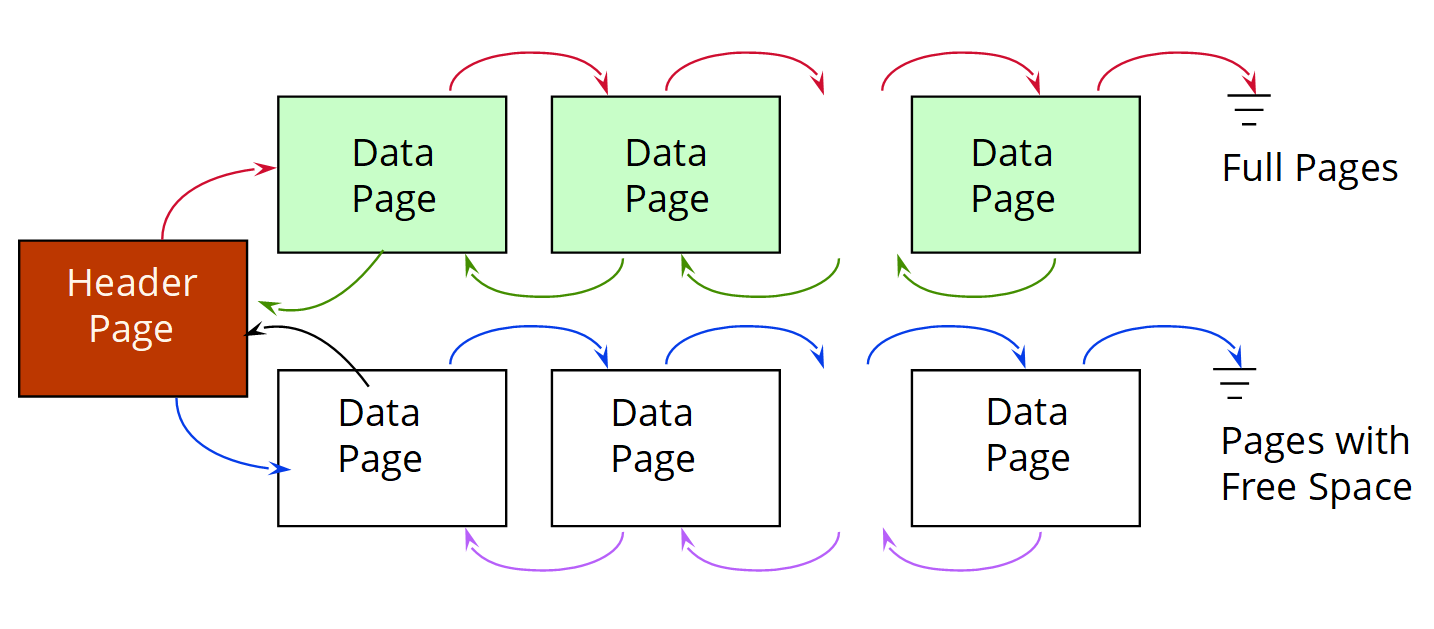
\includegraphics[width=.8\linewidth]{data-storage-architecture/heap-file-linked-list}
		\caption{Heap File: Linked List Implementation}
		\label{img:heap-file-linked-list}
	\end{figure}

& \textbf{Page directory heap file implementation:} Heap file implementation consisting of a linked list where each node contains a set of pointers to pages, and the amount of free space on the pages
	&& Allocation process: Search through nodes to find a page with enough space (reading only one page)
	&& Diagram: See figure~\ref{img:heap-file-page-directory}
		
	\begin{figure}[!htb]
		\centering
		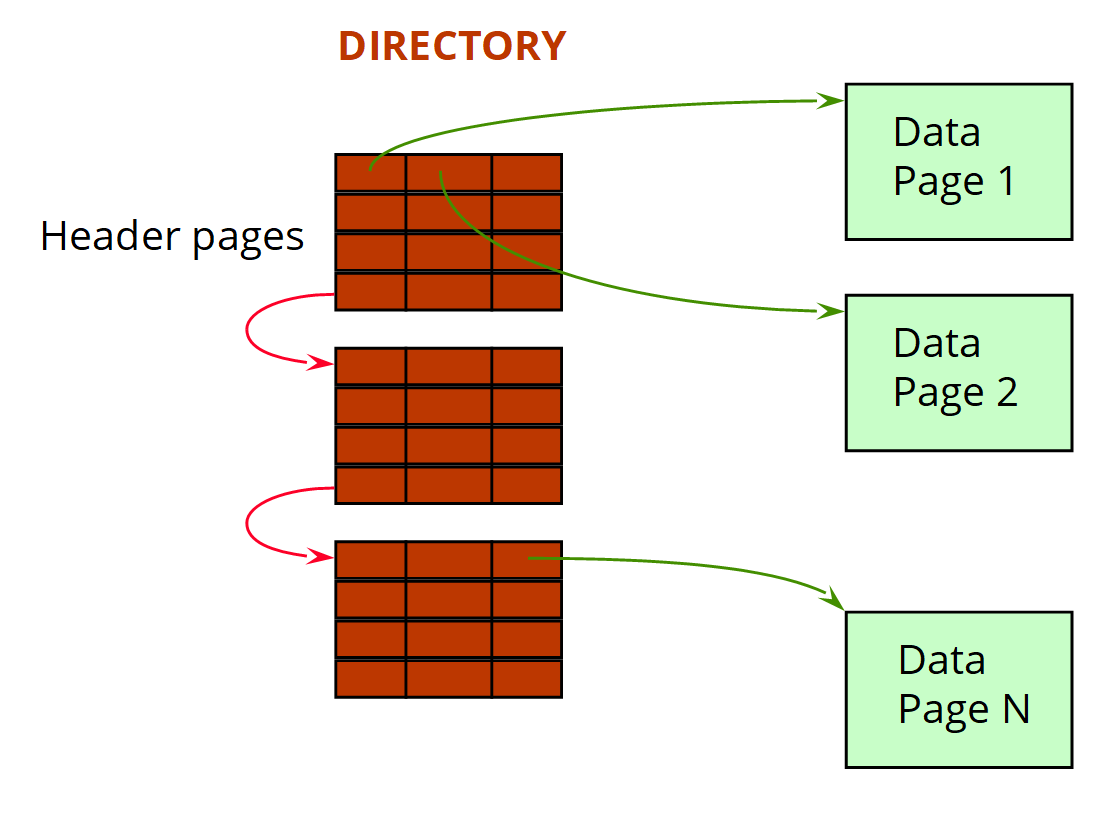
\includegraphics[width=.8\linewidth]{data-storage-architecture/heap-file-page-directory}
		\caption{Heap File: Page Directory Implementation}
		\label{img:heap-file-page-directory}
	\end{figure}

\end{easylist}
\clearpage